\section{Solution Methods}

A type of differential equations we have already dealt with is given by
equations of the form:
\[
   u'(x) = f(x).
\]
Trivially, the set of solutions is given by the antiderivatives of $f$:
\[
  u \in \int f.
\]
If $f$ is defined on an interval, all solutions are defined on the same interval
and, thanks to Theorem~\ref{th:primitive}, they can be written in the form
\[
  u(x) = F(x) + c
\]
where $F$ is any antiderivative of $f$ and $c\in \RR$ is an arbitrary additive
constant.
If $f$ is continuous and we consider the Cauchy problem:
\[
  \begin{cases}
    u'(x) = f(x) \\
    u(x_0) = y_0.
  \end{cases}
\]
we can identify a unique solution which is written in the form:
\[
  u(x) = y_0 + \int_{x_0}^x f(t)\, dt.
\]

\subsection{First Order Linear Equations}

First order ordinary differential equations in normal form can be written in the
form:
\mymark{***}
\begin{equation}\label{eq:47744}
   u'(x) + a(x) u(x) = b(x).
\end{equation}

To solve these equations, we try to reduce the sum on the left-hand side to the
derivative of a product.
To do this, we consider any antiderivative $A\in \int a$ and multiply both sides
by $e^{A(x)}$:
\[
  e^{A(x)} u'(x) + a(x) e^{A(x)} u(x) = b(x) e^{A(x)}
\]
since $A'(x) = a(x)$, we observe that the left-hand side is now the derivative
of a product:
\[
  \enclose{e^{A(x)}u(x)}' = b(x) e^{A(x)}
\]
from which
\[
  e^{A(x)} u(x) \in \int b(x) e^{A(x)}\, dx.
\]
Multiplying both sides by $e^{-A(x)}$ (since the exponential never vanishes,
this operation does not modify the solution space), we obtain
\[
u(x) = e^{-A(x)} \int b(x) e^{A(x)}\, dx, \qquad
A(x) \in \int a(x)\, dx.
\]

More explicitly, choosing any antiderivative of the right-hand side
\[
  F(x) \in \int b(x) \cdot e^{A(x)}\, dx
\]
on any interval where $a(x)$ and $b(x)$ are defined, we have
\[
  u(x) = e^{-A(x)}\cdot \enclose{F(x) + c}.
\]
for some $c\in \RR$.

If $b(x)=0$, the equation is homogeneous linear, we can choose $F(x) = 0$, and
thus the solution space in this case is given by
\[
  u(x) = c \cdot e^{-A(x)}
\]
and is therefore the one-dimensional vector space generated by the function
$e^{-A(x)}$.

Every solution of the non-homogeneous equation can be written as the sum of a
particular solution $u_0$ of the non-homogeneous equation plus a generic
solution of the associated homogeneous equation. Indeed:
\[
  u(x) = u_0(x) + c e^{-A(x)}
\]
where
\[
  u_0(x) = e^{-A(x)}F(x)
\]
is a particular solution of the non-homogeneous equation.

We observe that if $a(x)$ and $b(x)$ are continuous functions defined on the
same interval $I$, the solution is also defined on the entire $I$. It will
therefore be said that the solution exists \emph{globally}.

\begin{exercise}[Eigenvectors of the Derivative Operator]%
  \label{ex:58230978}
Given $\lambda \in \RR$, find all solutions of the equation
\[
  u'(x) = \lambda u(x).
\]
\end{exercise}
%
\begin{proof}[Solution]
We write the equation in the form
\[
  u'(x) - \lambda u(x) = 0.
\]
In the previous notations, we have $a(x) = -\lambda$, and thus we can choose
$A(x) = -\lambda x \in \int a$.
Multiplying both sides by $e^{A(x)}$, we obtain
\[
  e^{-\lambda x} u'(x) - \lambda e^{-\lambda x} u(x) = 0
\]
that is
\[
 \enclose{e^{-\lambda x}\cdot u(x)}' = 0
\]
from which, on every interval where $u$ is defined, there exists a constant $c$
such that
\[
  e^{-\lambda x} u(x) = c
\]
or
\[
  u(x) = c e^{\lambda x}.
\]
We have thus found that the solutions are defined on the entire $\RR$, one
solution is $e^{\lambda x}$, and every other solution is a multiple of this.
\end{proof}

\begin{exercise}
\begin{enumerate}
\item
Find the solutions of the differential equation
\[
  u' - \frac{u}{x} = x^2.
\]

\item
Find the solutions of the differential equation
\[
  x u' - u = x^3.
\]
\end{enumerate}
\end{exercise}
\begin{proof}[Solution]
The first is a non-homogeneous first-order linear equation of
type~\eqref{eq:47744}. The integrating factor is $e^{A(x)}$ with
\[
  A(x) \in \int a(x)\, dx = -\int \frac{1}{x}\, dx \ni - \ln \abs{x}.
\]
Thus $e^{A(x)} = 1/\abs{x}$. We should then divide both sides of the equation by
$\abs{x}$. We observe that the equation is not defined for $x=0$, and we can
thus distinguish the cases $x>0$ and $x<0$. We then decide, for simplicity, to
change the sign of the equation for $x<0$ so that we can divide by $x$ instead
of $\abs{x}$.
We thus obtain:
\[
  \frac{u'}{x} - \frac{u}{x^2} = x
\]
that is
\[
  \enclose{u\cdot \frac{1}{x}}'  = x
\]
from which
\[
  \frac{u}{x} \in \int x\, dx \ni \frac{x^2}{2}.
\]
Thus the function $u(x)/x$ differs from $x^2/2$ by a constant on each of the two
intervals $x>0$ and $x<0$. On each of the two intervals, we have:
\[
  \frac{u(x)}{x} = \frac{x^2}{2} + c
\]
from which
\[
  u(x) = \frac{x^3}{2} + c x
\]
for some $c\in \RR$. As posed, the solution need not be defined for $x=0$, and
the constant $c$ may be different if $x>0$ or $x<0$.

The second equation is equivalent to the first if $x\neq 0$. But it is not in
normal form, and the solutions may be defined even for $x=0$.
We will have
\[
  u(x) = \frac{x^3}{2} + c x
\]
as before, but for the function to be differentiable at $x=0$, the constant $c$
must be the same for $x>0$ and $x<0$.

Note that every solution satisfies the initial condition $u(0) = 0$, and thus no
solution satisfies the condition $u(0)= q$ if $q \neq 0$.
\end{proof}

\begin{exercise}
Solve the differential equation:
\[
 u' + \frac{u}{(1+x^2)\arctg x} = 1.
\]
\end{exercise}
%
\begin{proof}[Solution.]
We observe that the equation is defined only for $x\neq 0$. We will therefore
look for solutions on the two intervals $x<0$ and $x>0$.
Multiplying both sides of the equation by $\arctg x$, we obtain
\[
  \arctg x \cdot u'(x) +\frac{1}{1+x^2} u(x) = \arctg x
\]
that is:
\[
  \enclose{\arctg x \cdot u(x)}' = \arctg x
\]
from which
\[
  \arctg x \cdot u(x) \in \int \arctg x\, dx \ni x \arctg x - \frac {1}{2}\ln(1+x^2).
\]
Thus on each interval where the solution is defined, there will exist $c\in \RR$
such that
\[
  \arctg x \cdot u(x) = x \arctg x - \frac{1}{2}\ln(1+x^2) + c
\]
from which, since $x\neq 0$, we can divide by $\arctg x$ and obtain
\[
  u(x) = x - \frac{\ln(1+x^2)}{2\arctg x} + \frac{c}{\arctg x}.
\]
We thus have a family of solutions defined for $x<0$ and a family of solutions
defined for $x>0$.
\end{proof}

\subsection{Equations with Separable Variables}

Equations of the type:
\mymark{***}
\begin{equation}\label{eq:edo_separabile}
  u'(x) = f(x) \cdot g(u(x)).
\end{equation}
are called equations with separable variables.
This is a first-order equation in normal form:
\[
  u'(x) = F(x, u(x))
\]
where in the function $F$ it is possible to separate the two variables into a
product:
\[
  F(x, y) = f(x)\cdot g(y).
\]

If $u$ is a solution of equation~\eqref{eq:edo_separabile} and if $x$ is a point
where $g(u(x))\neq 0$, we can divide both sides of the equation by $g(u(x))$ to
obtain:
\[
  \frac{u'(x)}{g(u(x))} = f(x).
\]
We now want to write the left-hand side as the derivative of the composed
function. If we choose an antiderivative of $1/g$:
\[
  H(u) \in \int \frac{1}{g(u)}\, du
\]
we observe that
\[
  \enclose{H(u(x))}' = H'(u(x))\cdot u'(x) = \frac{u'(x)}{g(u(x))} = f(x).
\]
thus if $F\in \int f$, on every interval where $g(u(x))\neq 0$, there must exist
$c\in \RR$ such that
\[
  H(u(x)) = F(x) + c.
\]
If we also assume that $H$ is invertible, we will have:
\[
  u(x) = H^{-1}(F(x)+ c).
\]

\begin{example}
Solve the equation 
\begin{equation}\label{eq:separabile}
  u' = x^2 e^u.
\end{equation}
\end{example}
%
\begin{proof}[Solution.]
Since $e^u \neq 0$, we can divide both sides of the equation by $e^u$:
\[
  \frac{u'(x)}{e^{u(x)}} = x^2  
\]
taking the antiderivatives of both sides, we obtain
\[
 \int\frac{u'(x)}{e^{u(x)}}\, dx  = \int x^2\, dx 
\]
and making the change of variables: $u=u(x)$, $du = u'(x) dx$ 
we obtain:
\[
  \Enclose{\int e^{-u}\, \, du}_{u=u(x)} = \frac{x^3}{3} + c
\]
from which 
\[
  -e^{-u(x)} = \frac{x^3}{3} + c
\]
or $u(x) = -\ln\enclose{-c -  \frac{x^3}{3}}$.
Setting $b=-c$
we obtain 
\[
  u(x) = -\ln \enclose{b-\frac{x^3}{3}}.
\]
Thus for every $b\in \RR$, we obtain a solution 
$u\colon \openinterval{-\infty}{\sqrt[3]{3b}}\to \RR$.
\end{proof}
%
\newsavebox{\qrseparabile}\sbox{\qrseparabile}{%
\myqrshortdoclink{separabile}{the graphs of the solutions of the differential equation (\getrefnumber{eq:separabile})}}
\begin{figure}
\centering

\includegraphics[width=0.8\textwidth]{fig_edo_separabile.pdf}
\caption{the graphs of the solutions of the differential equation~\eqref{eq:separabile}.
Note that each solution has a vertical asymptote, thus the individual 
solutions are not defined on the entire $\RR$.
But given any point in the plane, there is a solution that passes through 
that point, and moreover, two different solutions never meet.
These properties are guaranteed by Theorem~\ref{th:banach-caccioppoli}.
\ifwidemargin\\\\\fi%
\usebox{\qrseparabile}}
\label{fig:separabile}
\end{figure}

\begin{example}
Solve the equation
\begin{equation}\label{eq:43856}
  u' = x u^2 + x.
\end{example}
%
\begin{proof}[Solution.]
It is a first-order equation in normal form.
By factoring $x$ on the right-hand side, we obtain an equation with separable
variables.
Dividing both sides by $u^2+1$ (which is always non-zero), we obtain the
equivalent equation
\[
\frac{u'}{1+u^2} = x.
\]
Integrating the left-hand side, we obtain:
\[
  \int \frac{u'(x)}{1+u^2(x)}\, dx
  = \Enclose{\int \frac{du}{1+u^2}}_{u=u(x)}
  \ni \arctg(u(x))
\]
while for the right-hand side, we obtain
\[
  \int x\, dx \ni \frac{x^2}{2}.
\]
Thus on every interval, there must exist a constant $c\in \RR$ such that
\[
  \arctg(u(x)) = \frac{x^2}{2} + c.
\]
Since the arctangent takes values between $-\pi/2$ and $\pi/2$, the right-hand
side must also remain in this interval. Therefore, it must be:
\begin{equation}\label{eq:4856}
  -\frac \pi 2 < \frac {x^2} 2 + c < \frac \pi 2 .
\end{equation}
With this condition, we can invert the arctangent, finally obtaining an
expression for the solution:
\begin{equation}\label{eq:45876314}
  u(x) = \tg\enclose{\frac{x^2}{2} + c}.
\end{equation}

\newsavebox{\qrquattrotre}\sbox{\qrquattrotre}{%
\myqrshortdoclink{43856}{the graphs of the solutions of the differential equation (\getrefnumber{eq:43856})}}
\begin{figure}
\centering
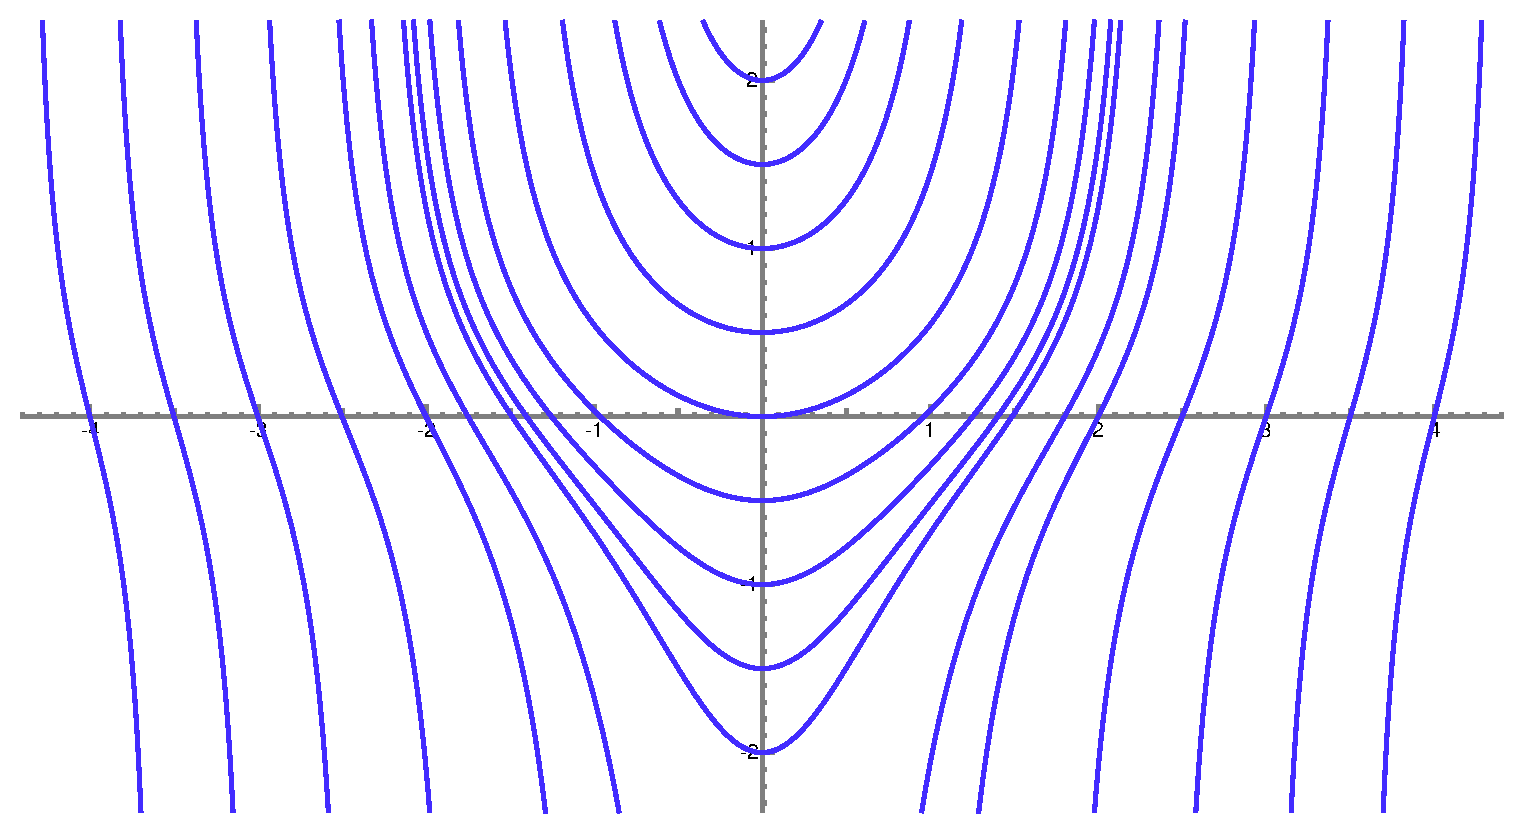
\includegraphics[width=0.8\textwidth]{fig_43856.pdf}
\caption{the graphs of the solutions of the differential equation~\eqref{eq:43856}.
\ifwidemargin\\\\\fi%
\usebox{\qrquattrotre}}
\label{fig:43856}
\end{figure}

We observe that condition~\eqref{eq:4856} is equivalent to requiring that the
argument of the tangent lies in the interval $\enclose{-\frac \pi 2, \frac \pi
2}$.
In such a case, it must be $c<\frac\pi 2$, and we observe that if $c>-\frac \pi
2$, the solution $u(x)$ is defined on an open interval centered at $x=0$, while
if $c \le -\frac \pi 2$, the solution is defined on a pair of symmetric
intervals with width tending to zero as $c\to -\infty$.
At the ends of these intervals, the solution has vertical asymptotes.

In this case, we can observe that condition~\eqref{eq:4856} can be disregarded
since the function $\tg$ is $\pi$-periodic, and therefore it is possible to add
an integer multiple of $\pi$ to $c$ without modifying the solution.
In equation~\eqref{eq:45876314}, one could thus consider the function $\tg$
defined over its entire domain, observing that in such a case, it can be assumed
that $c\in \left(-\frac \pi 2, \frac \pi 2\right]$.
Instead of obtaining a single interval for each $c$, one thus obtains all the
infinite intervals.
\end{proof}

\begin{remark}
The previous example highlights the fact that maximal solutions can be defined
on arbitrarily small intervals even if the differential equation does not
present singularities. In this case, we will say that the solution is not
global.

On the other hand, we observe that the graphs of the solutions fill the entire
plane without ever touching each other (sometimes said to be a
\emph{fibration}).
This is due to the fact that this equation satisfies
Theorem~\ref{th:cauchy_lipschitz}, and therefore, through every point of the
plane, there passes one and only one solution.
\end{remark}

\begin{example}
Consider solving the equation
\[
  u' = u^2.
\]
This is a first-order equation in normal form, autonomous.
In particular, it is separable
$u' = f(u(x))\cdot g(x)$
with $f(u)=u^2$ and $g(x)=1$.
We first observe that $u(x) = 0$ is a solution since $u'(x) = u^2(x) = 0$.
If $u$ is a solution not identically zero, there will be points where
$u(x)\neq 0$.
In a neighborhood of such points, we can divide both sides of the equation by
$u^2(x)$, obtaining:
\[
  \frac{u'}{u^2} = 1.
\]
Integrating the left-hand side by changing variables $u=u(x)$, $du=u'(x)\, dx$,
we obtain:
\[
  \int \frac{u'(x)}{u^2(x)}\, dx = \Enclose{\int \frac{du}{u^2}}_{u=u(x)} = \Enclose{-\frac{1}{u}}_{u=u(x)}
  = -\frac{1}{u(x)}
\]
while integrating the right-hand side, we have
\[
  \int 1 \, dx \ni x.
\]
Thus on every interval where $u(x)\neq 0$, there must exist a constant $c\in
\RR$ such that
\[
-\frac{1}{u(x)} = x + c
\]
or, setting $x_0 = -c$
\begin{equation}\label{eq:5782196}
  u(x) = -\frac{1}{x+c} = \frac{1}{x_0-x}.
\end{equation}

In conclusion, we have found a constant solution $u(x)=0$ and a family of
solutions defined on the intervals $(-\infty,x_0)$ and $(x_0,+\infty)$
represented by equation~\eqref{eq:5782196}.
We should now ask ourselves whether it is possible for these solutions to be
mixed together, i.e., if a solution can be zero in some regions and
satisfy~\eqref{eq:5782196} in others.

In this case, the answer is no.
It suffices to observe that a function $u$ satisfying
equation~\eqref{eq:5782196} can tend to zero only when $x\to +\infty$ or $x\to
-\infty$.
This means that if we consider a solution $u(x)$ defined on an interval $I$ and
if at least at one point the solution is different from zero, then the solution
is different from zero on the entire $I$ and satisfies
equation~\eqref{eq:5782196} since the null solution and the solution
\eqref{eq:5782196} are not compatible with each other (they cannot be glued
together continuously).

We will see later a result (Proposition~\ref{prop:separazione_soluzioni}) that
guarantees in very general hypotheses that two different solutions can never
meet.
\end{example}

\begin{exercise}
Given $p>1$, solve the differential equation
\[
  u' = u^p
\]
and observe that the solution always presents a vertical asymptote (thus there
is no global existence).
\end{exercise}

\begin{example}[Peano's Mustache]
Determine all solutions of the Cauchy problem
\begin{equation}
\label{eq:94467}
\begin{cases}
  u'(x) = \sqrt[3]{u(x)}\\
  u(0)=0
\end{cases}
\end{equation}
\end{example}
%
\newsavebox{\qrnovequattro}\sbox{\qrnovequattro}{%
\myqrshortdoclink{94467}{Peano's mustache formed by the solutions of the Cauchy problem (\getrefnumber{eq:94467})}}
\begin{figure}
\centering
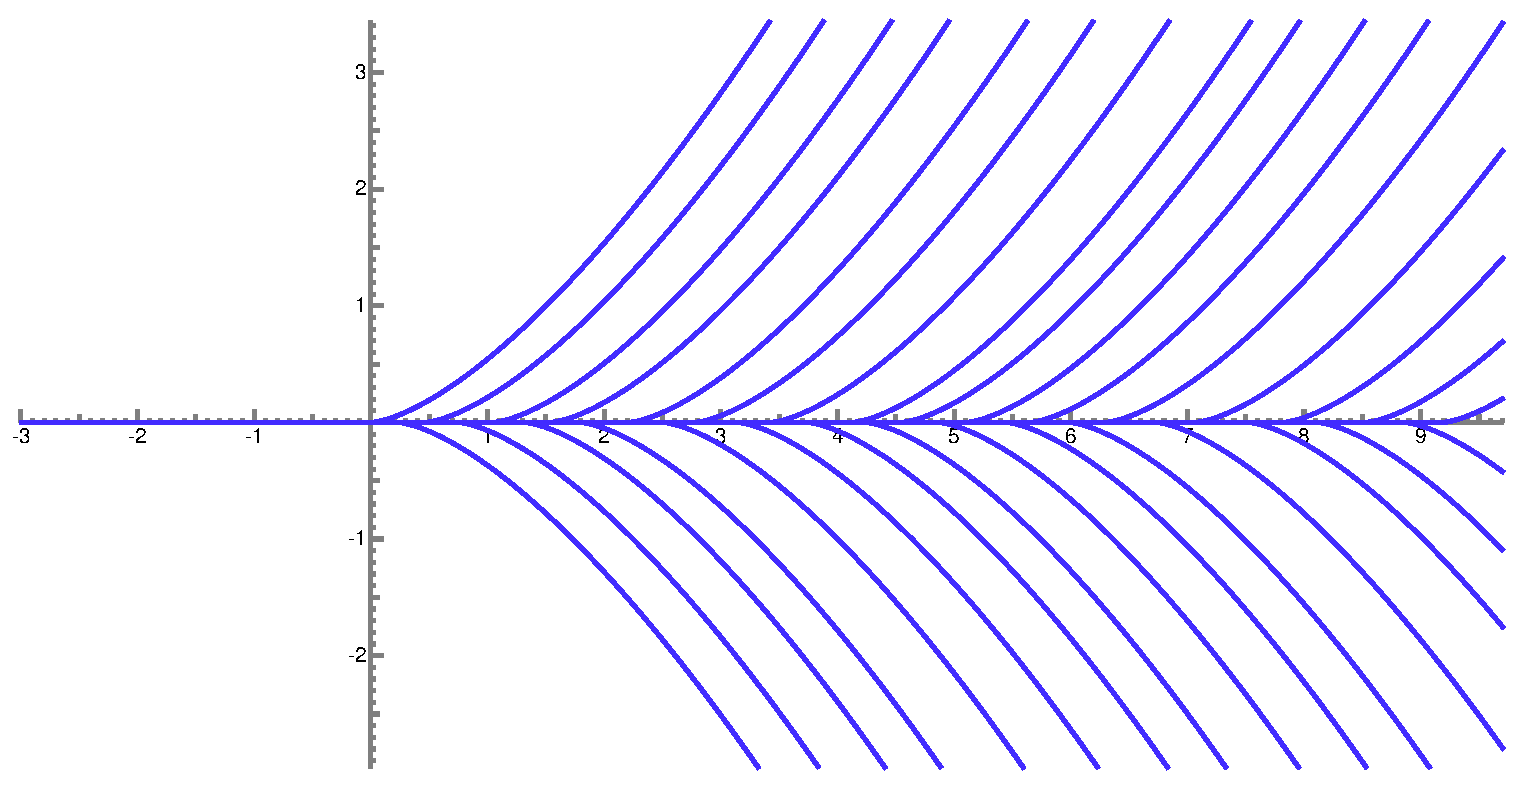
\includegraphics[width=0.9\textwidth]{fig_94467.pdf}
\caption{Peano's mustache formed by the solutions of the Cauchy problem~\eqref{eq:94467}.\\\\
\usebox{\qrnovequattro}}
\label{fig:94467}
\end{figure}
%
\begin{proof}[Solution.]
We observe that the null function $u(x)=0$ is a solution of the equation and
satisfies the condition $u(0)=0$.
But a priori, we cannot exclude that there are other solutions of the equation
that verify the same condition (we will see that
Proposition~\ref{prop:separazione_soluzioni} does not apply in this particular
case).

In points where $u(x)\neq 0$, we can rewrite the equation in the form
\[
  \frac{u'(x)}{\sqrt[3]{u(x)}} = 1.
\]
Integrating the left-hand side by changing variables $u=u(x)$, $du = u'(x)\,
dx$, we obtain
\[
  \int \frac{u'(x)}{\sqrt[3]{u(x)}}\, dx
  = \Enclose{\int \frac{du}{\sqrt[3]u}}_{u=u(x)}
  \ni \frac 3 2 \sqrt[3]{u^2(x)}.
\]
Integrating the right-hand side, we find that on every interval where $u$ is
defined and $u(x)\neq 0$, there must exist a constant $c$ such that
\[
  \frac 3 2 \sqrt[3]{u^2(x)} = x + c.
\]
Solving for $u(x)$:
\begin{equation}\label{eq:476937568}
  u(x) = \pm \sqrt{\enclose{\frac 2 3 (x+c)}^3}.
\end{equation}
We observe that the previous property can only be satisfied if $x\ge -c$, but
for $u(x)\neq 0$, we must impose $x>-c$.
But for $x\to -c^+$, we have $u(x)\to 0$ and also $u'(x) = \sqrt[3]{u(x)}\to 0$.
This means that a solution defined on $x>c$ by equation~\eqref{eq:476937568} can
be extended to the entire $\RR$ by setting $u(x)=0$ for $x\le c$.
To satisfy the condition $u(0)=0$, it will therefore be sufficient to impose the
restriction $-c\ge 0$.

Our problem thus has infinite solutions defined on the entire $\RR$.
Specifically, for each $c\ge 0$ (we change the sign of the constant found before
so that it is positive), we have the solutions
\[
  u(x) = \begin{cases}
    0 & \text{for $x\le c$}\\
    \sqrt{\enclose{\frac 2 3 (x-c)}^3} & \text{for $x>c$}
  \end{cases}
\]
and
\[
  u(x) = \begin{cases}
    0 & \text{for $x\le c$}\\
    -\sqrt{\enclose{\frac 2 3 (x-c)}^3} & \text{for $x>c$}
  \end{cases}
\]
\end{proof}
\subsection{Other Solution Methods}

In the previous section, we saw that first-order linear equations and equations
with separable variables can be reduced to the calculation of an antiderivative.
In Section~\ref{sec:edo_lineari}, solution methods for linear equations of order
$n$ with constant coefficients will be presented.

There are many other types of equations that can be reduced to linear equations
or equations with separable variables.
We cannot dwell on these methods, but it may be useful, as a non-exhaustive
reference, to list some types of equations for which a solution method exists.

\begin{enumerate}
\item \emph{Second-order equation without dependence on $u$}
\[
  F(x, u', u'') = 0
\]
is reduced to first order by setting $u'(x) = v(x)$, $u''(x) = v'(x)$.

\item \emph{Autonomous second-order equation}
\[
  F(u, u', u'') = 0
\]
is reduced to first order by setting $u'(x) = v(u(x))$, $u''(x) = v'(u(x))\cdot
v(u(x))$.

\item \emph{First-order homogeneous equations}
\index{equation!homogeneous}%
\[
  u' = h(x,u(x))
\]
where $h$ is homogeneous, i.e., $h(tx,ty)=h(x,y)$ for every $t\in \RR$.
It is reduced to an equation with separable variables by making the substitution
$u(x) = x\cdot v(x)$.

\item \emph{Bernoulli's equation}
\index{equation!Bernoulli's}%
\index{Bernoulli!equation of}%
\[
  u' = a(x) u + b(x) u^\alpha
\]
is reduced to a linear equation by dividing everything by $u^\alpha$ and setting
$u(x)^{1-\alpha} = v(x)$, $\frac{u'}{u^\alpha} = \frac{v'}{1-\alpha}$.

\item \emph{Clairaut's equation}
\index{equation!Clairaut's}%
\index{Clairaut!equation of}%
\[
  u = x u' + f(u');
\]
by differentiating the equation, we obtain $ u' = u' + xu'' + f'(u')u''$, which
factors: $u''\cdot(x+f'(u'))=0$.
The second factor allows us to determine $u'(x)$, and by inserting $u'$ into the
original equation, we find $u(x)$.
The first factor $u''=0$ gives us a solution that is a line, which, by
substituting its equation into the original equation, we discover to be tangent
to the solution found previously.
To these solutions, we must add the non-$C^2$ solutions formed by a segment of
the initial curve that then detaches along the tangent half-lines.

\item \emph{Riccati's equation}
\index{equation!Riccati's}%
\index{Riccati!equation of}%
\[
  u' = u^2 + b(x) u + c(x).
\]
set $u(x) = -v'(x)/v(x)$ to reduce to a second-order linear equation in $v$:
\[
 v'' -  b(x) v' + c v = 0.
\]
\end{enumerate}

\begin{example}[Newton's Equation]
\index{equation!Newton's}%
\index{Newton!equation of}%
A one-dimensional physical system subject to forces that depend only on position
can be described by a Cauchy problem:
\[
\begin{cases}
  u''(x) = F(u(x)) \\
  u(x_0) = u_0 \\
  u'(x_0) = v_0
\end{cases}
\]
(for example, for the pendulum, we have $F(y) = -\sin y$).
The function $v$ defined by $v(u(x)) = u'(x)$ relates velocity to position and
thus describes the motion in the so-called \emph{phase space}. With this
substitution, we find
\[
  u''(x) = v'(u(x)) u'(x) = v'(u(x)) v(u(x))
\]
which, substituted into $u'' = F(u)$, gives us a first-order differential
equation for $v=v(u)$:
\[
 v' v  = F(u).
\]
This is a first-order equation with separable variables that can be interpreted
as the law of conservation of energy, as it is equivalent to
\[
  \frac{d}{dx}\enclose{\frac 1 2 v^2 - \int F(u)} = 0
\]
where $\frac 1 2 v^2$ is interpreted as kinetic energy and $-\int F$ as
potential energy.
Integrating between $x_0$ and $x$ and using the initial conditions, we obtain,
with $u=u(x)$:
\[
  \frac 1 2 v^2(u) = \frac 1 2 v_0^2 + \int_{u_0}^{u} F(y)\, dy.
\]
This equation describes the trajectory of the system in the phase plane $(u,v)$
and allows us to derive $v$ as a function of $u$:
\[
  v(u) = \pm\sqrt{v_0^2 + 2\int_{u_0}^u F(u)\, du}
\]
which means:
\begin{equation}\label{eq:8844475}
  u'(x) = \pm \sqrt{v_0^2 + 2 \int_{u_0}^{u(x)} F(y)\, dy}.
\end{equation}
This is an autonomous equation in $u$, thus with separable variables:
\[
  \pm\frac{u'(x)}{\sqrt{v_0^2 - \int_{u_0}^{u(x)} F(y)\, dy}} = 1
\]
which can be integrated between $x_0$ and $x$ by changing variables $u=u(x)$
\[
  \pm\int_{u_0}^{u(x)} \frac{du}{\sqrt{v_0^2-\int_{u_0}^u F(y)\, dy}} = x-x_0.
\]
In this way, we have determined the inverse function of the solution $u(x)$.
\end{example}

\begin{example}[Period of the Pendulum]
\index{period!pendulum's}%
\index{pendulum!period of the}%
\index{oscillations!small of the pendulum}%
\index{small oscillations}%
Let's try to determine the period of oscillation of a pendulum.
\end{example}
\begin{proof}[Solution.]
Let $u(x)$ be the angle of deviation from the vertical at time $x$ of a simple
pendulum of length $\ell$.
Considering the tangential component of gravitational acceleration (whose
magnitude is $g$), Newton's equation can be written in the form:
\[
  u''(x) = -\frac{g}{\ell} \sin u(x).
\]
We are thus in the case of the previous example where $F(u) = -\frac{g}{\ell}
\sin u$, and if at time $x=0$ we let the pendulum fall from rest from an angle
$u_0$, we will have $v_0=0$. The potential energy will then be given by
\[
-\frac{g}{\ell}\int_{u_0}^u \sin y\, dy = \frac{g}{\ell}\enclose{\cos u - \cos
u_0}.
\]
Equation~\eqref{eq:8844475} thus becomes
\[
  u'(x) = \pm \sqrt{2\frac{g}{\ell}(\cos u(x) - \cos u_0)}.
\]
Separating the variables and integrating between $0$ and $x$, we obtain
\[
\sqrt{\frac \ell g}\int_0^x \frac{u'(t)\, dt}{\pm\sqrt{2\cos u(t)-2\cos u_0}}
= \int_0^x dt  = x.
\]
Changing variables $u=u(x)$, $du = u'(x) dx$:
\begin{equation}\label{eq:4898944}
\sqrt{\frac \ell g}\int_0^{u(x)} \frac{du}{\pm\sqrt{2\cos u-2\cos u_0}} = x.
\end{equation}
The choice of the sign $\pm$ is arbitrary, but since $u$ is continuous,
$u''=-\frac g l \sin u$ must also be a continuous function. Thus the sign $\pm$
can only change when $u'=0$. At the initial point $x=0$, we imposed $u'(0) = 0$,
and thus the kinetic energy is zero. Since kinetic energy cannot be negative, it
means that potential energy cannot increase, and therefore initially the angle
$u(x)$ must decrease (or at least: it cannot increase). Thus initially the sign
of $u'$ is negative and will remain negative until $u'(x)=0$ again.
The integral in~\eqref{eq:4898944} is an improper integral since the integrand
function presents an asymptote for $u\to u_0^-$; we must therefore ensure that
the integral is finite. Expanding $\cos u$ at the point $u=u_0$, we find $\cos u
= \cos u_0  - \sin u_0 \cdot (u-u_0) + o(u-u_0)$ from which
\[
 \frac{1}{\sqrt{2 \cos u - 2 \cos u_0}}
 =\frac{1}{\sqrt{2\sin u_0\cdot (u_0-u) + o(u-u_0)}}
 \sim \frac{C}{\sqrt{u_0-u}}
\]
which is notoriously an integrable function for $u\to u_0^-$.

We now want to calculate the time $x_1$ at which the pendulum first reaches the
vertical, i.e., $u(x_1)=0$.
Recall that at time $x=0$, the pendulum starts from an angle $u_0$ with zero
velocity. In the interval $x\in[0,x_1]$, we will have $u'(x)<0$ (the angle
decreases), thus:
\[
-\sqrt{\frac{\ell}{g}}\int_{u_0}^{0} \frac{du}{\sqrt{2\cos u - 2\cos u_0}}
= x_1.
\]

Once it reaches the vertical, by symmetry, the pendulum will rise again to an
angle $-u_0$, taking the same time $x_1$. Then it will descend again and rise
until it returns to the angle $u_0$, taking a total time $T=4x_1$, which is
therefore the period of oscillation. We have thus
\[
  \frac{T}{4} = \sqrt{\frac \ell g}\int_0^{u_0} \frac{du}{\sqrt{2\cos u - 2\cos u_0}}.
\]

Unfortunately, the integral we have found does not have an antiderivative
expressible in terms of elementary functions (it is an elliptic integral).
Our goal is now to make a Taylor expansion for $u_0\to 0$, which means
determining the period of the pendulum for \emph{small oscillations}%
\mymargin{small oscillations}\index{small oscillations}.

Using bisection formulas, we can write $\cos u = 1 - 2 \sin^2\frac u 2$, from
which
\[
 \sqrt{2\cos u - 2\cos u_0}
 = \sqrt{4\sin^2 \frac {u_0} 2 - 4 \sin^2 \frac{u}{2}}
  = 2\sin \frac{u_0}2 \sqrt{1-\enclose{\frac{\sin \frac u 2}{\sin \frac
 {u_0}2}}^2}
\]
thus setting
\begin{equation}\label{eq:4847843}
 \sin t = \frac{\sin \frac u 2}{\sin \frac{u_0} 2}
\end{equation}
we have
\[
  \sqrt{\frac \ell g} \cdot \frac T 4
  =  \int_0^{u_0} \frac{du}{2\sin \frac {u_0}2 \sqrt{1-\sin^2 t}}
  = \int_0^{u_0} \frac{du}{2\sin \frac{u_0}2 \cos t}
\]
but for the change of variable~\eqref{eq:4847843}, we have
\[
  \cos t \, dt = \frac{\cos \frac u 2 }{2 \sin \frac{u_0} 2}\, du
\]
or
\[
 \frac{du}{2\sin \frac {u_0} 2 \cos t} = \frac{dt}{\cos \frac u 2}
 = \frac{dt}{\sqrt{1-\sin^2 t \sin^2\frac{u_0}{2}}}
\]
and therefore
\[
\sqrt{\frac g \ell} \cdot \frac{T}{4}
= \int_0^{\frac \pi 2} \frac{dt}{\cos \frac u 2}
= \int_0^{\frac \pi 2} \frac{dt}{\sqrt{1-\sin^2 \frac u 2}}
= \int_0^{\frac \pi 2} \frac{dt}{\sqrt{1-\sin^2 \frac{u_0}{2} \sin^2 t}}.
\]
Now using the binomial series (Theorem~\ref{th:serie_binomiale}), we can write
\begin{align*}
\sqrt{\frac g \ell} \cdot\frac{T}{4}
&= \int_0^{\frac \pi 2} \sum_{k=0}^{+\infty}{-\frac 1 2 \choose k}
\enclose{-\sin^2 t\sin^2 \frac{u_0}2}^{k}\, dt
\end{align*}
\begin{align*}
&= \int_0^{\frac \pi 2} \sum_{k=0}^{+\infty}\frac{(2k-1)!!}{(2k)!!}
\enclose{\sin^2 t\sin^2 \frac{u_0}2}^{k}\, dt
\end{align*}
since we have
\begin{align*}
  {-\frac 1 2 \choose k}
    &= \frac{\enclose{-\frac 1 2}\cdot \enclose{-\frac 3 2} \cdots
  \enclose{-\frac{2k-1} 2}}{k!}\\
  &= (-1)^k\frac{(2k-1)!!}{2^k \cdot k!} = (-1)^k \frac{(2k-1)!!}{(2k)!!}.
\end{align*}
With respect to the variable $\sin^2 t$ inside the integral, we now have a power
series with coefficients
\[
 a_k = \frac{(2k-1)!!}{(2k)!!} \enclose{\sin^2\frac{u_0} 2}^{k}
\]
and it is easily verified that
$  \frac{a_{k+1}}{a_k} \to \sin^2 \frac{u_0}{2}$
thus the power series converges if
$ \sin^2 t \le \frac{1}{\sin^2 \frac{u_0}{2}}$
which simply means
$ \sin \frac u 2 < 1$.
We are thus performing an integral strictly within the radius of convergence of
the series.
We know that the series converges totally and therefore uniformly on this
interval.
Thus, applying Theorem~\ref{th:scambio_limite_integrale} to the partial sums of
the series, we can exchange the series with the integral:
\[
\sqrt{\frac g \ell} \cdot\frac{T}{4}
= \sum_{k=0}^{+\infty}\frac{(2k-1)!!}{(2k)!!} \enclose{\sin \frac{u_0}2}^{2k}
\int_0^{\frac \pi 2}  \enclose{\sin t}^{2k}\, dt
\]
the integral is now essentially the same $I_n$ that we calculated in
Theorem~\ref{th:wallis}:
\[
  \int_0^{\frac \pi 2} \enclose{\sin t}^{2k}\, dt
  = \frac 1 2 \int_0^{\pi} \enclose{\sin t}^{2k}\, dt
  = \frac{I_{2k}}{2}
  = \frac \pi 2 \cdot\frac{(2k-1)!!}{(2k)!!}
\]
from which
\[
T
= 2\pi\sqrt{\frac \ell g}\sum_{k=0}^{+\infty} \enclose{\frac{(2k-1)!!}{(2k)!}}^2
\enclose{\sin \frac{u_0} 2}^{2k}.
\]

We can then try to write the first terms of the Taylor expansion of $T = T(u_0)$
for $u_0\to 0$, say, for example, up to order 8 in $u_0$. It will suffice to
consider the sum of the terms of the series for $k=0,1,2,3,4$ since the sum of
the terms for $k\ge 5$ will give me a contribution of the order of
$O\enclose{\sin \frac {u_0} 2}^{10} = o(u_0^8)$. Thus
 \begin{align*}
 \sqrt{\frac{g}{\ell}}\cdot \frac{T}{2\pi}
 &=
 1 + \enclose{\frac 1 2}^2 \sin^2 \frac{u_0} 2
 + \enclose{\frac{1\cdot 3}{2\cdot 4}}^2\enclose{\sin^2 \frac {u_0} 2}^2 \\
 &\quad + \enclose{\frac{1\cdot 3 \cdot 5}{2\cdot 4 \cdot 6}}^2
 \enclose{\sin^2 \frac {u_0} 2}^3 + \enclose{\frac{1\cdot 3\cdot 5 \cdot 7}{2\cdot 4\cdot 6\cdot 8}}^2
 \enclose{\sin^2 \frac {u_0} 2}^4 + o(u_0^8) \\
%\end{align*}
%\begin{align*}
 &=
1 + \frac 1 4 \enclose{\frac{u_0^2}{4} - \frac{u_0^4}{2^4\cdot 3} +
\frac{u_0^6}{2^5\cdot 3^2\cdot 5}
- \frac{u_0^8}{2^8\cdot 3^2\cdot 5\cdot 7}} \\
&\quad + \frac{3^2}{2^6}\enclose{\frac{u_0^2}{4} - \frac{u_0^4}{2^4\cdot 3}
+ \frac{u_0^6}{2^5\cdot 3^2\cdot 5}}^2\\
&\quad + \frac{5^2}{2^8}\enclose{\frac{u_0^2}{4} - \frac{u_0^4}{2^4\cdot 3}}^3
+ \frac{5^2\cdot 7^2}{2^{14}}
\frac {u_0^8} {2^8} + o(u_0^8)\\
%\end{align*}
%\begin{align*}
&=
1 + \frac{u_0^2}{2^4} - \frac{u_0^4}{2^6\cdot 3} + \frac{u_0^6}{2^7\cdot
3^2\cdot 5}
- \frac{u_0^8}{2^{10}\cdot 3^2\cdot 5\cdot 7} \\
&\quad + \frac{3^2}{2^6}\enclose{\frac{u_0^4}{2^4} - \frac{u_0^6}{2^5\cdot 3} +
\frac{u_0^8}{2^8\cdot 3^2} + \frac{u_0^8}{2^6\cdot 3^2\cdot 5}}\\
&\quad + \frac{5^2}{2^8}\enclose{\frac{u_0^6}{2^6} - \frac{u_0^8}{2^8}}
+ \frac{5^2\cdot 7^2}{2^{22}}
u_0^8 + o(u_0^8)\\
%
% \end{align*}
% \begin{align*}
&= 1 + \frac{u_0^2}{2^4} + \frac{11}{2^{10}\cdot 3} u_0^4
 + \frac{173}{2^{14}\cdot 3^2\cdot 5} u_0^6
 + \frac{22931}{2^{22}\cdot 3^2\cdot 5\cdot 7} u_0^8
 + o(u_0^8).\\
\end{align*}
\end{proof}

%%%%%%%%%%%%%%%%%%%%
%%%%%%%%%%%%%%%%%%%%
%%%%%%%%%%%%%%%%%%%%
\section[Vector and Multivariable Functions]{Some Preparatory Results on Vector and Multivariable Functions}
%%%%%%%%%%%%%%%%%%%%
%%%%%%%%%%%%%%%%%%%%
%%%%%%%%%%%%%%%%%%%%

It will be useful to extend the definition of $C^k$ regularity classes to vector
functions (i.e., with codomain $\RR^n$) and multivariable functions (i.e., with
domain $\RR^m$).

\subsection{Continuity and Compactness}

The space $\RR^n$ is a metric space with the Euclidean distance
(Definition~\ref{def:124124})
$d(\vec x, \vec y) = \abs{\vec x- \vec y}$ with 
\[
 \abs{\vec x} = \sqrt{x_1^2 + \dots + x_n^2}.  
\] 

Thus, a sequence $\vec x_k\in \RR^n$ converges to a point $\vec p\in \RR^n$ if
(Definition~\ref{def:convergenza_metrica})
$\abs{\vec x_k - \vec p}\to 0$.
If $(x_k)_j$ are the components of the point $\vec x_k\in \RR^n$ and 
$p_j$ are the components of $\vec p\in \RR^n$, the convergence 
$\vec x_k \to \vec p$ is equivalent to the convergence of 
all components: $(x_k)_j \to p_j$ for every $j=1,\dots,n$
as $k\to +\infty$.

A function $\vec f\colon A \subset \RR^n\to \RR^m$ 
is \emph{continuous} 
(Definition~\ref{def:continua_metrico})
if for every sequence $\vec x_n \to \vec p$ with 
$\vec x_n\in A$ and $\vec p\in A$, it holds that 
\[
  \vec f(\vec x_n) \to \vec f(\vec p).
\]

A set $K\subset \RR^n$ is \emph{closed}%
\mymargin{closed}\index{closed}
if given any convergent sequence in $\RR^n$: $\vec x_k \to \vec x$, if every
$\vec x_k\in K$, then also
$\vec x \in K$ (i.e., $K$ is closed under taking limits,
Theorem~\ref{th:chiuso_sequenziale}).
The ball of radius $r>0$ centered at the point $\vec p\in \RR^n$ 
is the set (Definition~\ref{def:palla}):
\[
  B_r(\vec p) = \ENCLOSE{\vec x \in \RR^n\colon \abs{\vec x - \vec p}< r}.  
\]
A set $\Omega\subset \RR^n$ is \emph{open}
if for every $\vec p\in \Omega$, there exists $r>0$ such that $B_\rho(\vec p)
\subset \Omega$
(Definition~\ref{def:466342}).
A set $B\subset \RR^n$ is said to be \emph{bounded}
(Definition~\ref{def:spazio_limitato})
if there exists $r>0$ and $\vec p\in\RR^n$ such that $B\subset B_r(\vec p)$ 
(but it is not restrictive to assume $\vec p=0$).
A set $K\subset \RR^n$ is said to be \emph{compact} 
(Definition \ref{def:sequenzialmente_compatto}) if from every sequence 
$\vec x_k$ of points in $K$, it is possible to extract a subsequence $x_{k_j}
\to \vec x$
converging to a point $\vec x \in K$.
In $\RR^n$, a set is compact if and only if it is closed and bounded
(Theorem~\ref{th:compattezza_Rn}).
A continuous function $f\colon K\subset \RR^n\to\RR$ defined
on a compact $K$ is bounded by the Weierstrass theorem
(Theorem~\ref{th:weiestrass_metrico}).


\subsection{Partial Derivatives}

If $\Omega\subset \RR^m$ is an open set and $f\colon \Omega \to \RR$
is a function, we want to define the \emph{partial derivatives} of $f$.
If $\vec x \in \Omega$, we have $\vec x = (x_1,\dots, x_m)$, and therefore
$f(\vec x) = f(x_1,\dots, x_m)$. If we vary only one component
$x_j$ while keeping all other components fixed, we obtain a function
of one variable $x_j \mapsto g(x_j) = f(x_1,\dots, x_j, \dots, x_m)$.
We then define the \emph{partial derivative}
\mymargin{partial derivative}
\index{derivative!partial}
of $f$ with respect to the variable $x_j$ as the derivative of the function
$g(x_j)$.
We denote this derivative with the symbol:
\[
  \frac{\partial f}{\partial x_j}.
\]
Partial derivatives are thus calculated as usual derivatives for functions of
one variable, only considering all variables as constants except the one
involved in the differentiation.
For example, if $f(x,v) = -\sin(x) - v$
(as in the example made in the introduction), we have
\begin{align*}
  \frac{\partial f}{\partial x} &= -\cos(x)\\
  \frac{\partial f}{\partial v} &= -1.
\end{align*}

If $\vec f\colon \Omega \subset \RR^m \to \RR^n$ is a function of multiple
variables with vector values, we can write $\vec f = (f_1, \dots, f_n)$
and consider the partial derivatives of each component:
\[
  \frac{\partial \vec f}{\partial x_j}
    = \enclose{\frac{\partial f_1}{\partial x_j}, \dots, \frac{\partial
  f_n}{\partial x_j}}.
\]

\begin{definition}
Let $\Omega\subset \RR^m$ be an open set. We denote by $C^0(\Omega,\RR^n)$
the vector space of all continuous functions
$f\colon \Omega \to \RR^n$.

We denote by $C^1(\Omega,\RR^n)$ the vector space
of functions in $C^0(\Omega,\RR^n)$ such that each of their partial derivatives
$\frac{\partial f}{\partial x_j}$ exists at every point of $\Omega$ and
is itself a continuous function (i.e., in $C^0(\Omega,\RR^n)$).
Recursively, $C^k(\Omega,\RR^n)$ is defined for $k>1$,
as the space of functions $\Omega\to\RR^n$ such that all their partial
derivatives are in $C^{k-1}(\Omega,\RR^n)$.

When the target space is not indicated, it is always understood to be $\RR$, so
$C^k(\Omega) = C^k(\Omega,\RR)$.
\end{definition}

\begin{theorem}[Stability of Regular Functions]
Let $\Omega \subset \RR^n$ be an open set.
If $f,g\in C^k(\Omega)$, then $f+g$, $f-g$, $f\cdot g$, and $\frac{f}{g}$
(where defined) are also of class $C^k$. If $f\in C^k(\Omega)$ and $g\in
C^k(\RR)$,
then $g\circ f \in C^k(\Omega)$.
\end{theorem}
%
\begin{proof}
The fact that the composition of continuous functions is a continuous function
is true in general in any metric space.
Indeed, if $f\colon X\to Y$ and $g\colon Y \to Z$ and if $x_k\to x$ in $X$,
then $f(x_k) \to f(x)$ in $Y$ (by the continuity of $f$)
and therefore $g(f(x_k)) \to g(f(x))$ in $Z$ (by the continuity of $g$).
Thus $(g \circ f)(x_k) \to (g\circ f)(x)$ and $g\circ f\colon X\to Z$ is
continuous.

We can thus observe that the functions of two variables $s(x,y) = x+y$,
$d(x,y)=x-y$, and
$m(x,y)=xy$ are continuous functions from $\RR^2\to \RR$ 
(thanks to Theorem~\ref{th:operazioni_limiti}). 
This guarantees
that the sum, difference, and product of continuous functions are continuous
functions.
Also, the reciprocal of continuous functions is a continuous function
since the function $r(x)=1/x$ is continuous.
It follows that the ratio of continuous functions is a
continuous function.

Now let's consider partial derivatives.
For the rules of differentiation of functions of one variable, we know that
the sum, product, difference, ratio (where defined), and composition
of differentiable functions are
themselves differentiable functions, and the derivative is always expressed
through
sum, product, difference, and ratio of the functions involved and their
derivatives. Thus what is obtained by combining functions
of class $C^k$ is a continuous function whose partial derivatives exist and
are of class $C^{k-1}$, thus it is a function of class $C^k$.
\end{proof}

\subsection{Integrals of Vector Functions}

\begin{definition}
Let $\vec f\colon [a,b]\to \RR^m$, $\vec f(x) = (f_1(x), \dots, f_m(x))$.
We say that $\vec f$ is integrable on $[a,b]$ if each
$f_k\colon[a,b]\to \RR$ is integrable on $[a,b]$, and in such a case, we set:
\[
  \int_a^b \vec f(x)\, dx
  = \enclose{\int_a^b f_1(x)\, dx, \dots, \int_a^b f_m(x)\, dx}
  \in \RR^m
\]
so that for each $k=1,\dots, m$, we have:
\[
  \enclose{\int_a^b \vec f(x)\, dx}_k = \int_a^b f_k(x)\, dx.
\]
As usual, we also set $\int_b^a \vec f = - \int_a^b \vec f$.
\end{definition}

\begin{theorem}\label{teo:tipo_jensen}
\label{th:stima_modulo_integrale}%
\mymark{*}%
Let $\vec f\colon [a,b]\to \RR^m$ be integrable. Then we have
\[
  \abs{\int_a^b \vec f(x)\, dx} \le \int_a^b \abs{\vec f(x)}\, dx.
\]
\end{theorem}
%
\begin{proof}
Let
\[
 \vec v = \int_a^b \vec f(x)\, dx
\]
we have, using the linearity of the integral
and exploiting the Cauchy-Schwarz inequality
\begin{align*}
  \abs{\vec v}^2
  &= \vec v \cdot \vec v
   = \sum_{k=1}^m v_k \int_a^b f_k(x)\, dx
   = \int_a^b \sum_{k=1}^m v_k f_k(x)\, dx \\
  &= \int_a^b \enclose{\vec v, \vec f(x)}\, dx
  \le \int_a^b \abs{\vec v}\cdot \abs{\vec f(x)}\, dx
  = \abs{\vec v} \int_a^b \abs{\vec f(x)}\, dx.
\end{align*}
If $\abs{\vec v}\neq 0$, we can divide both sides by $\abs{\vec v}$ and
obtain the desired inequality.
Otherwise, if $\abs{\vec v}=0$, the inequality is certainly satisfied since
the right-hand side cannot be negative.
\end{proof}